\chapter{Project and Data Preparation}

\vspace*{0.3cm}

The project workflow starts with the raw instruction-following dataset and ends
with optimizer comparison for Edge AI analysis. Figure~\ref{fig:project_workflow}
summarizes the full pipeline, including data preparation, instruction formatting,
model loading, fine-tuning, evaluation, and future compression analysis.

\begin{figure}[H]
    \centering
    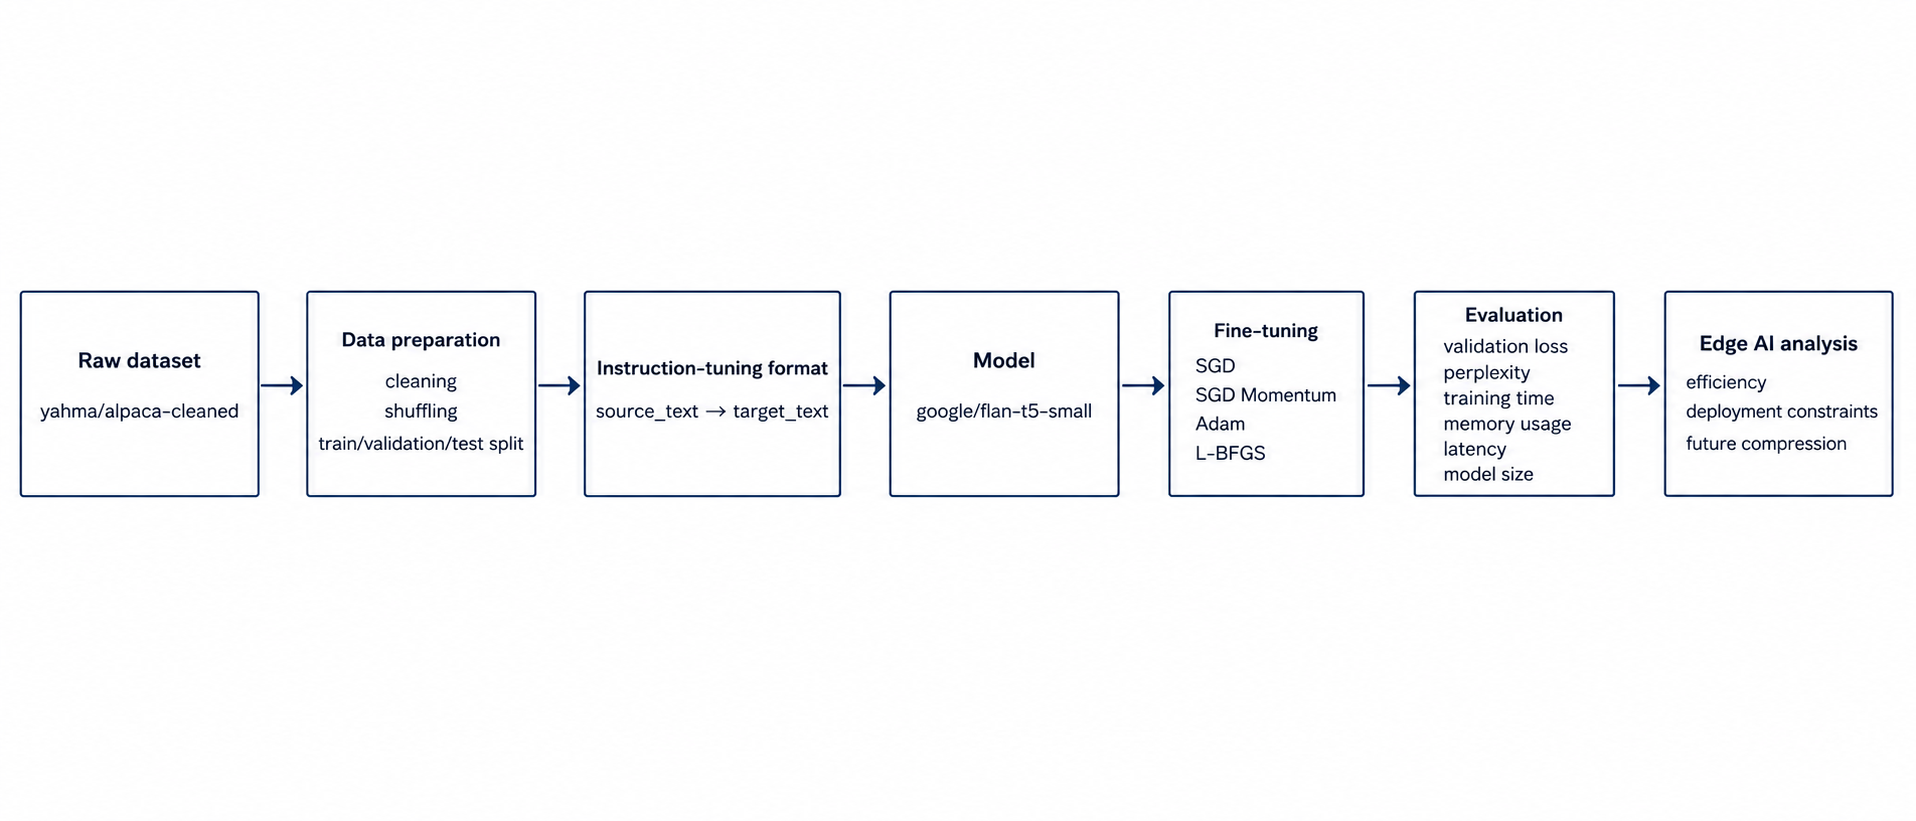
\includegraphics[width=\textwidth]{chapters/images/project_flow.png}
    \caption{General workflow of the project.}
    \label{fig:project_workflow}
\end{figure}

The dataset used is \texttt{yahma/alpaca-cleaned}, downloaded using the Hugging
Face \texttt{datasets} library \cite{alpaca}. Each example contains an
instruction, an optional input, and an output. This structure is appropriate for
instruction tuning because the model learns to generate an answer from a natural
language prompt. Figure~\ref{fig:dataset_examples} shows examples extracted from
the dataset.

\begin{figure}[H]
    \centering
    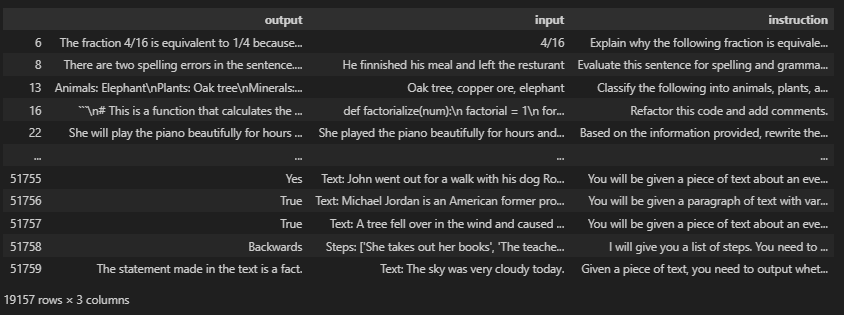
\includegraphics[width=0.95\textwidth]{chapters/images/dataset_examples.png}
    \caption{Examples extracted from the original instruction-following dataset.}
    \label{fig:dataset_examples}
\end{figure}

The data preparation configuration is stored in \texttt{config.yaml}. The
processed dataset contains 2000 training examples, 500 validation examples, and
500 test examples, with seed 42 for reproducibility. The processed files are
saved in \texttt{data/processed/} as \texttt{CSV} and \texttt{JSONL} files.

\begin{figure}[H]
    \centering
    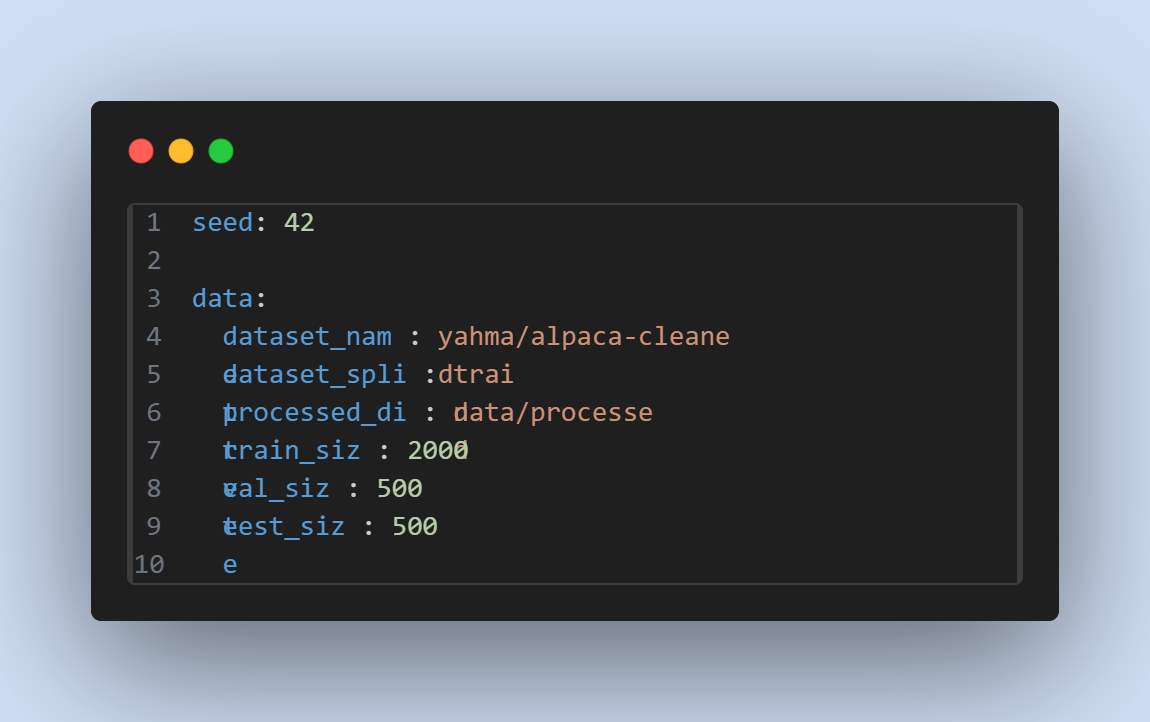
\includegraphics[width=0.8\textwidth]{chapters/images/config-yaml.png}
    \caption{Configuration file used for data preparation.}
    \label{fig:yaml_config}
\end{figure}

The preprocessing script \texttt{src/prepare\_data.py} loads the configuration,
downloads and shuffles the dataset, creates the train/validation/test subsets,
cleans empty fields, converts the data into instruction-tuning format, and saves
the processed files. The final model input is stored in \texttt{source\_text},
while the expected answer is stored in \texttt{target\_text}. If an example has
an input, the prompt contains the instruction, the input, and the keyword
\texttt{Answer:}. If no input is available, the prompt contains only the
instruction and \texttt{Answer:}.

\begin{figure}[H]
    \centering
    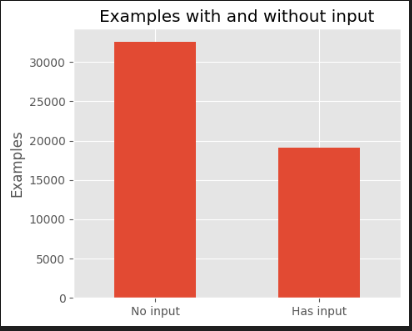
\includegraphics[width=0.5\textwidth]{chapters/images/input_distribution.png}
    \caption{Distribution of examples with and without input in the dataset.}
    \label{fig:input_distribution}
\end{figure}

\begin{table}[H]
    \centering
    \begin{tabular}{lr}
        \toprule
        \textbf{Statistic} & \textbf{Value} \\
        \midrule
        Original examples & 51760 \\
        Training examples & 2000 \\
        Validation examples & 500 \\
        Test examples & 500 \\
        Average source length & 17.14 words \\
        Average target length & 109.21 words \\
        Maximum source length & 279 words \\
        Maximum target length & 450 words \\
        \bottomrule
    \end{tabular}
    \caption{Statistics of the processed dataset.}
    \label{tab:data_stats}
\end{table}
